\chapter{Localization system} \label{chap:localization-system}



\section*{}

This chapter details the \gls{ros} implementation of the proposed 3/6 \gls{dof} self-localization system\footnote{\url{https://github.com/carlosmccosta/dynamic_robot_localization}}. It starts with an overview of the main processing stages and then details the control flow and algorithms within the localization pipeline.



\section{Overview}

The self-localization system was implemented as a \gls{ros} package and provides 3/6 \gls{dof} localization by publishing \emph{geometry\_msgs::PoseStamped}\footnote{\url{http://docs.ros.org/api/geometry_msgs/html/msg/PoseStamped.html}} and \emph{geometry\_msgs::TransformStamped}\footnote{\url{http://docs.ros.org/api/geometry_msgs/html/msg/TransformStamped.html}} messages along with a detailed analysis of the pose estimation and registered point cloud (split into inliers and outliers).

The system can receive sensor data through \emph{sensor\_msgs::PointCloud2}\footnote{\url{http://docs.ros.org/api/sensor_msgs/html/msg/PointCloud2.html}} messages and as a result it can directly use data from RGB-D and \gls{tof} cameras. To use \glspl{lidar} it provides an assembler that can produce point clouds by merging measurements from several sensors using spherical interpolation. As such, if the \gls{lidar} sensors are mounted on tilting platforms, they can emulate a 3D sensor and retrieve a very detailed view of the environment.

The self-localization system has a modular software architecture and was implemented as several C++ templated shared libraries that can be easily used for other applications besides robot self-localization. As can be seen in \cref{fig:localization-system_localization-system-overview}, it is an extensible and flexible system able to fit the needs of a wide range of mobile platforms. It can be configured as a tracking system, with or without pose recovery and can also have initial pose estimation using feature detection and matching. Moreover, it can also dynamically create and update the map if necessary.

To allow fast deployment of robots in large environments it supports two configurable processing pipelines. One to process new reference maps and another to localize a mobile robot platform using ambient point clouds. This enables the loading of either processed or unprocessed referenced point clouds and allows a navigation supervisor to dynamically provide the relevant map sections based on the robot position (in order to reduce the computation resources needed).

The next sections explain in detail the architecture and algorithms used in each of the processing modules present in \cref{fig:localization-system_localization-system-overview}.


\begin{figure}[H]
	\centering
	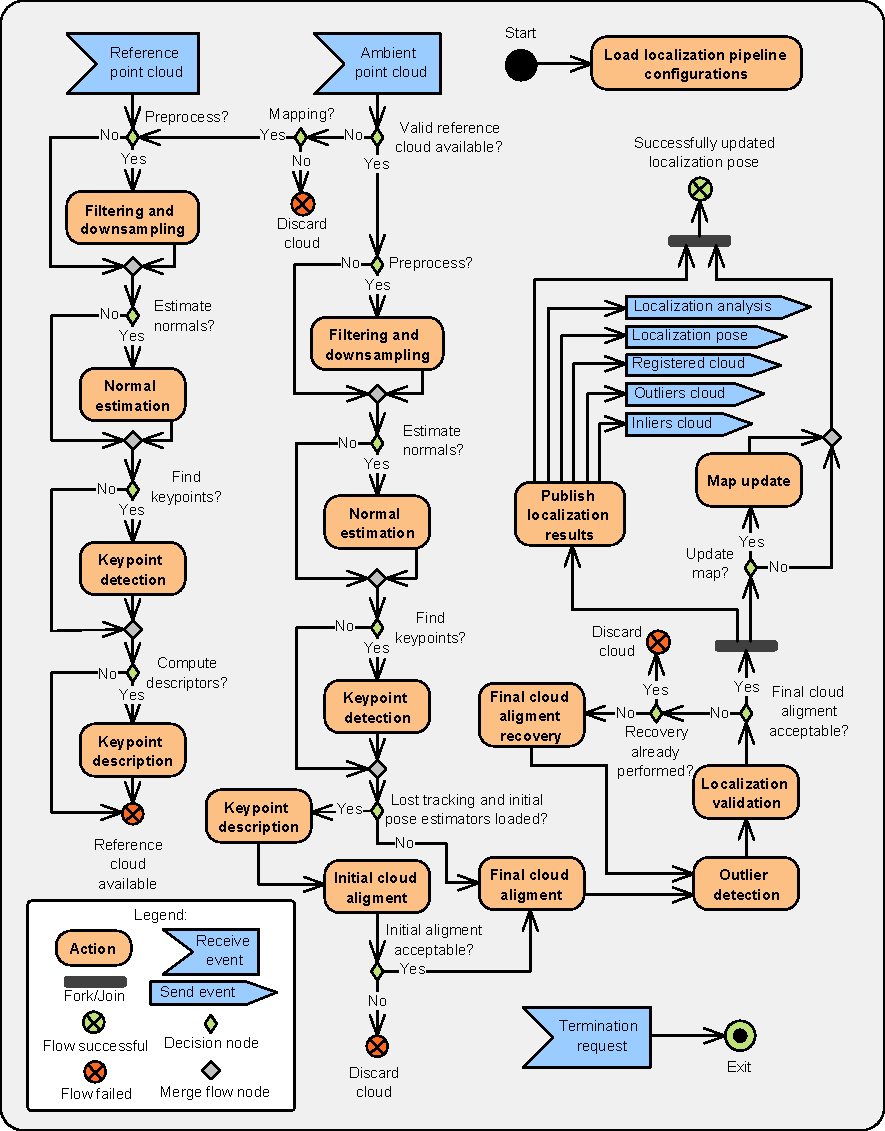
\includegraphics[width=\textwidth]{localization-system/localization-system-overview}
	\caption{Localization system overview}
	\label{fig:localization-system_localization-system-overview}
\end{figure}



\section{Pipeline configuration}

The self-localization system was designed to allow fast reconfiguration\footnote{\url{https://github.com/carlosmccosta/dynamic_robot_localization/blob/hydro-devel/yaml/schema/drl_configs.yaml}} and parameterization through the use of yaml\footnote{\url{http://yaml.org/}} files and the \gls{ros} parameter server\footnote{\url{http://wiki.ros.org/Parameter\%20Server}}. This gives the possibility to quickly tune the localization system to the specific needs of a given mobile platform moving in a particular environment, in order to use the least amount of computational resources possible and without requiring any reprogramming or source code modification. Nevertheless, the system can use a generic configuration if hardware resources are not a concern.

In a typical configuration (following the \emph{Yes} paths of the activity diagram in \cref{fig:localization-system_localization-system-overview}), the first time the localization system is used, it receives a raw reference point cloud that is preprocessed and saved to long term memory along with its associated keypoints and keypoint descriptors. This allows a much faster startup the next time the localization system is initialized. After having a reference point cloud, the localization system will estimate the robot pose periodically by analyzing the ambient point cloud sensor data. This data can be preprocessed with several filters and can be associated with computed surface normals. The robot pose estimation is performed by applying a matrix transformation correction to the current robot pose and is based on the registration of the ambient point cloud with the know map. This registration can use a tracking algorithm configuration tuned for efficiency and a second configuration for tracking recovery purposes. These tracking algorithms require a initial pose estimation, and as such, if one isn't available, a third configuration can be employed to estimate the global position of the robot based on geometric features of the environment. The switch between these configuration is based on the analysis of the registered cloud metrics, such as outlier percentage, inliers root mean square error, inliers angular distribution and the registration corrections performed to the ambient point cloud. After successfully performing the robot pose estimation, the map can be updated by either integrating the full registered point cloud, its inliers or its outliers. Finally, like most \gls{ros} nodes, the localization system will stop its execution when it receives a termination signal request.



\section{Point cloud assembly}

The self-localization system can use any sensor that provides point clouds, namely RGB-D / \gls{tof} cameras and \glspl{lidar}. Each of these types of sensors have very different operation rates as well as the amount of points that are produced in each environment analysis.



\section{Point cloud search data structures}

Most of the point cloud algorithms use neighbor searches to analyze the surroundings of a given point. As such, efficient data structures are needed to speedup these operations, in order to execute the algorithms efficiently.


\subsection{Voxel grids}

A voxel grid is a three dimensional space partition data structure that splits the Euclidean space into regular voxels (volume pixel). It can be built very fast but is not very efficient for sparse point clouds. \Cref{fig:point-cloud-algorithms_voxel-grid} shows how the voxel size affects the level of detail of point clouds.

\begin{figure}[H]
	\centering
	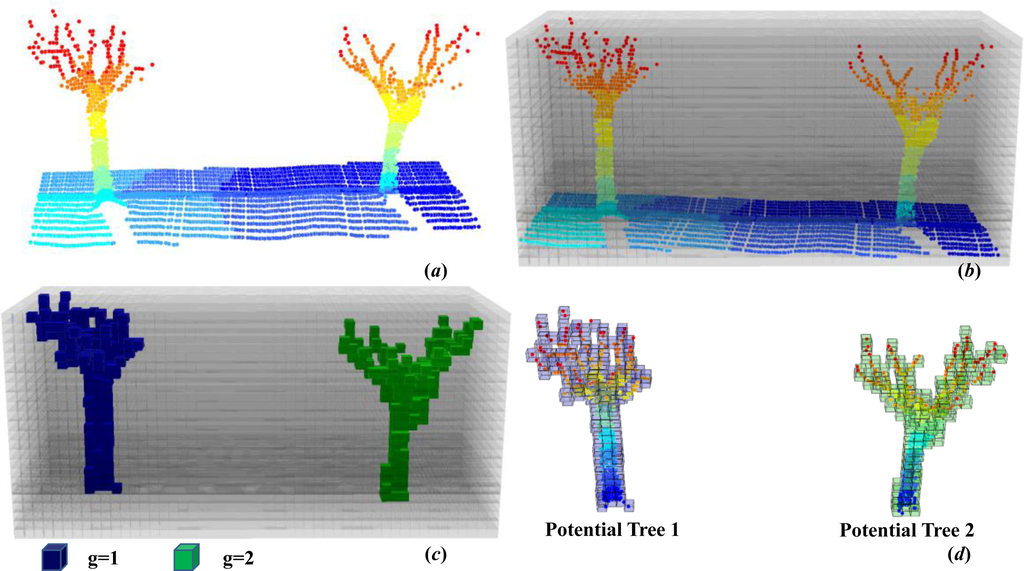
\includegraphics[width=\textwidth]{localization-system/voxel-grid}
	\caption[Voxel grid applied over trees point clouds]{Voxel grid applied over trees point clouds \cite{Wu2013}}
	\label{fig:point-cloud-algorithms_voxel-grid}
\end{figure}



\subsection{Octrees}

An octrees is a hierarchical space partition technique that adapts its tree data structure to the distribution of points in the cloud. It accomplishes this by recursively dividing each voxel in 8 octants until the tree depth is reached or when there is no more points in that region of space. This can be seen in \cref{fig:point-cloud-algorithms_octree} in which areas with no points have large voxels while areas with high point density have much smaller voxels.

%\afterpage{
\begin{figure}[H]
	\centering
	\begin{minipage}[h]{.495\textwidth}
		\centering
		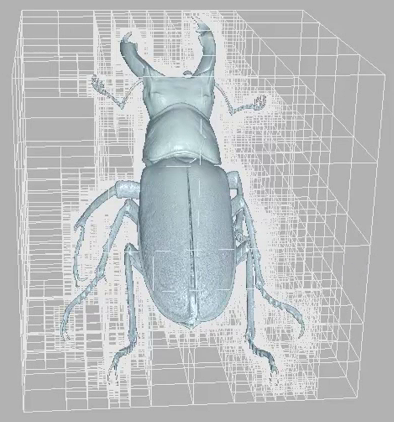
\includegraphics[width=0.55\textwidth]{localization-system/octree-1}
	\end{minipage}\hfill
	\begin{minipage}[h]{.495\textwidth}
		\centering
		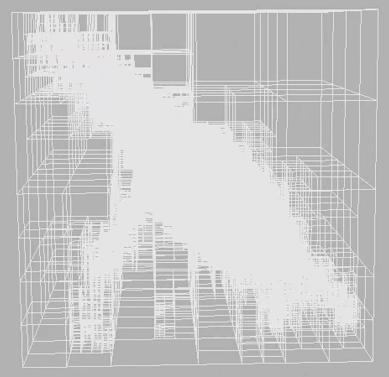
\includegraphics[width=0.6\textwidth]{localization-system/octree-2}
	\end{minipage}
	\caption[Octree of a stag beetle]{Octree of a stag beetle\protect\footnotemark}
	\label{fig:point-cloud-algorithms_octree}
\end{figure}
\footnotetext{\url{http://blog.mpanknin.de/?p=753}}
%}



\subsection{k-d trees}

A k dimensional tree is a space partition technique that can organize points with k dimensions. It is a generic data structure that can be used for 2D and 3D points (examples in \cref{fig:point-cloud-algorithms_2d-tree} and \cref{fig:point-cloud-algorithms_3d-tree}) as well as any other type of data that have an arbitrary number of dimensions (such as point cloud feature descriptors).

The binary k-d tree is built by successively selecting the median point in each axis until all points are inserted in the tree (the selection of the next axis is performed in a circular way, which in the case of three dimensional data means that after processing the z axis, the x axis would be selected).

%\afterpage{
\begin{savenotes}
\begin{figure}[H]
	\centering
	\begin{minipage}[h]{0.495\textwidth}
		\centering
		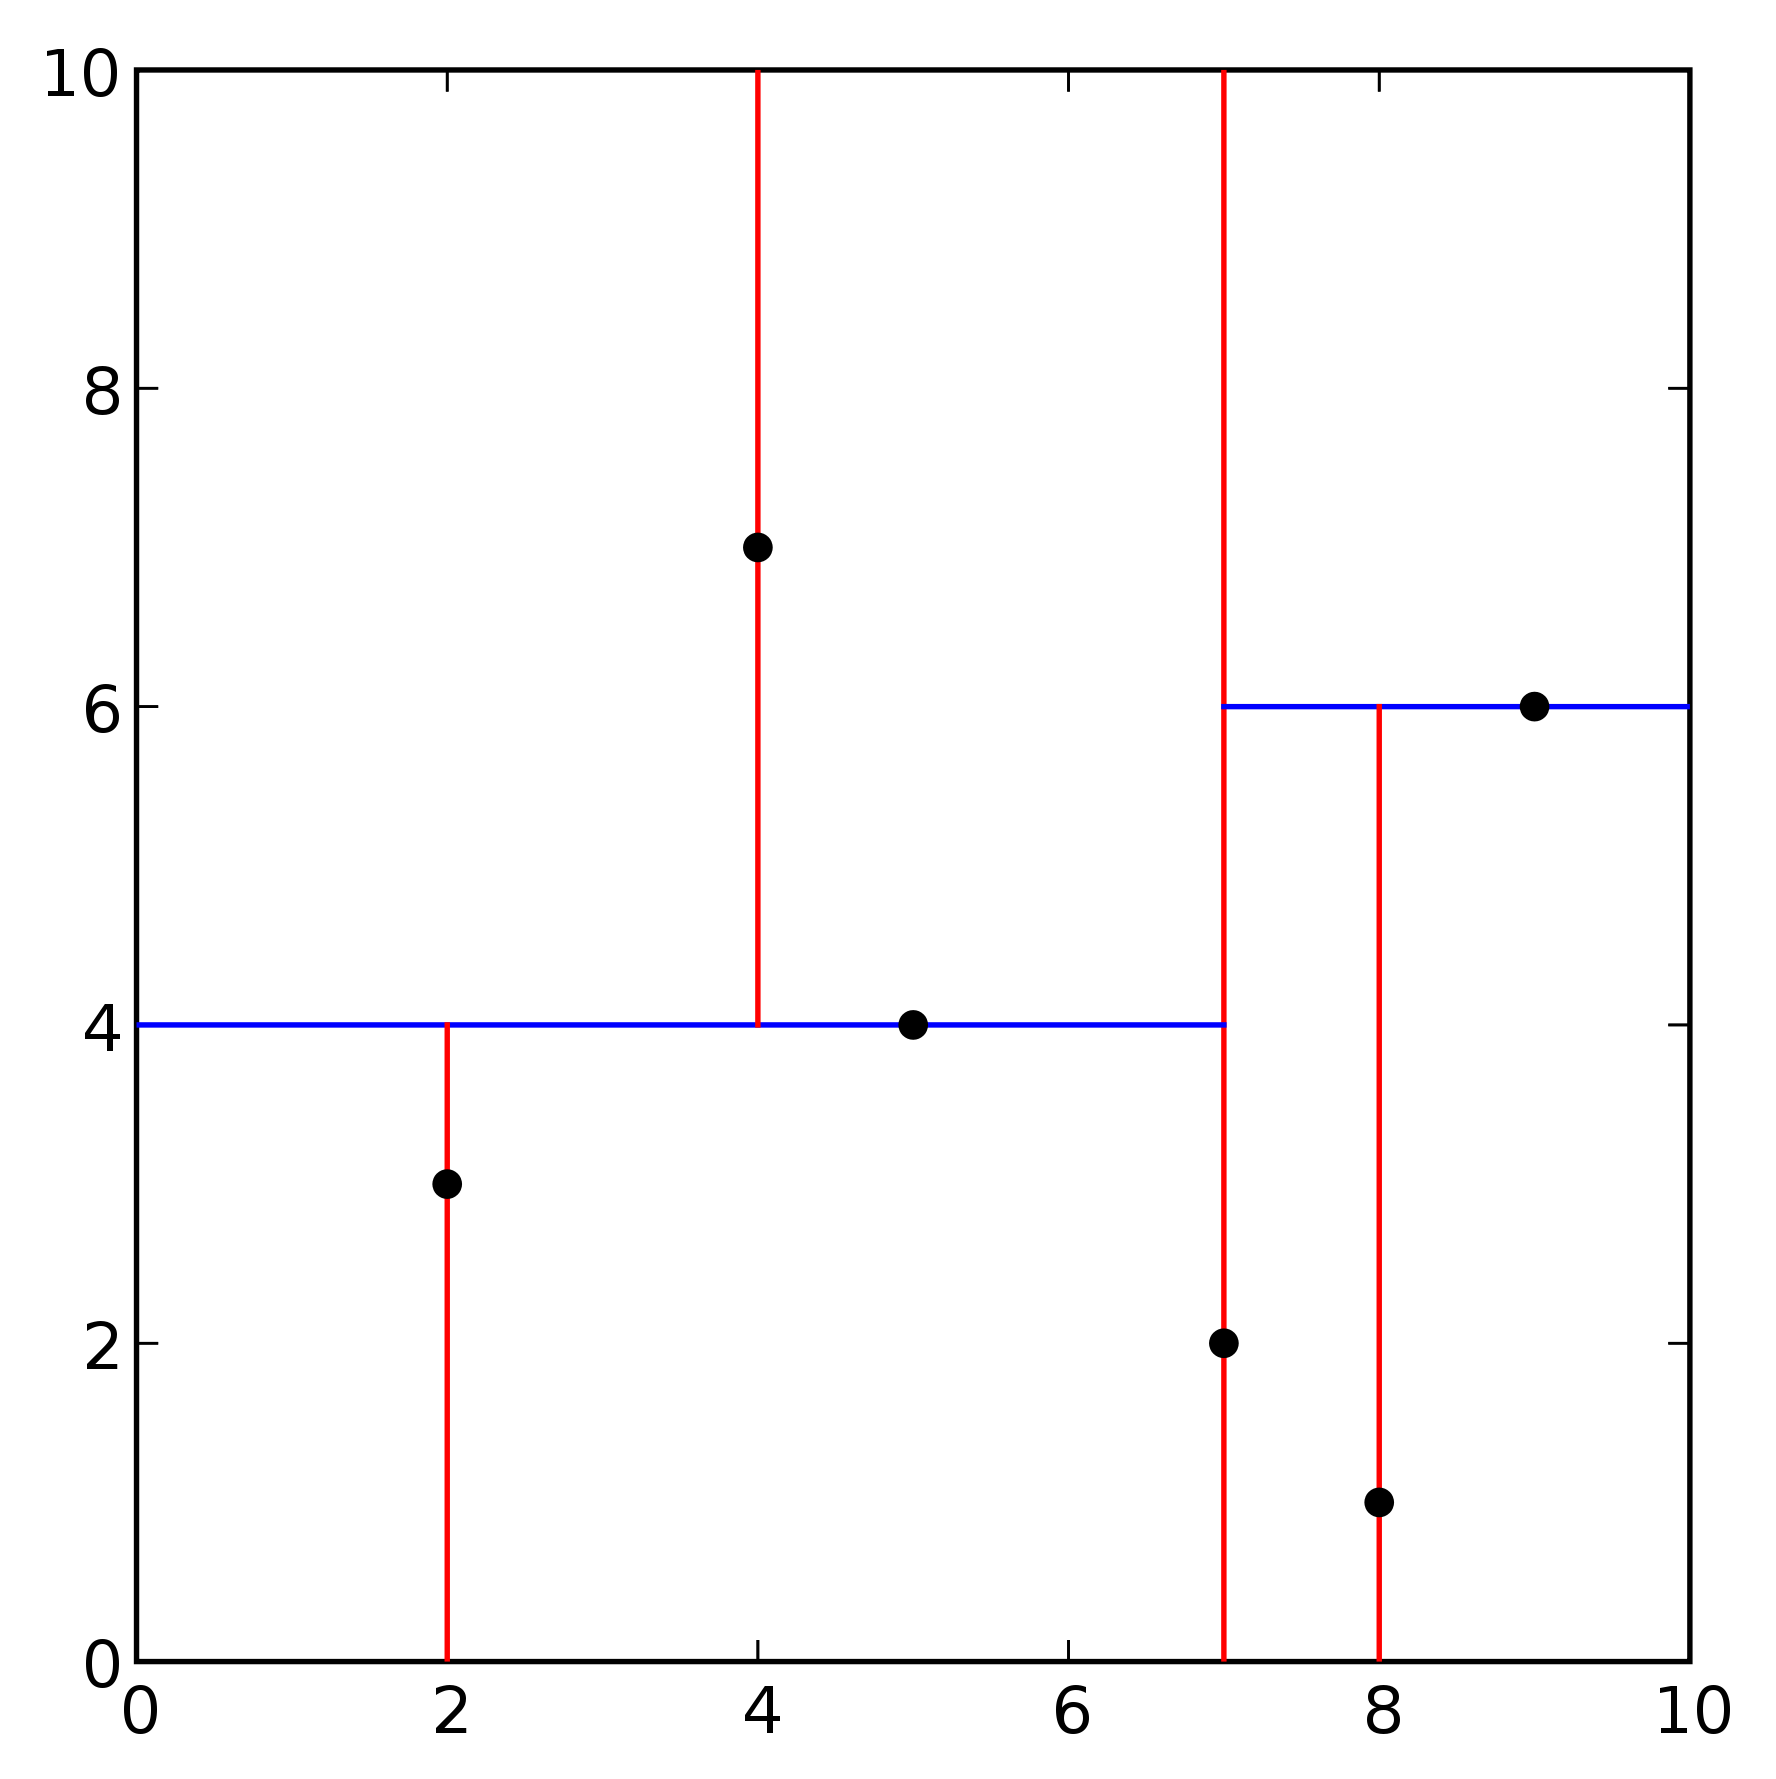
\includegraphics[width=0.6\textwidth]{localization-system/kdtree-2d}
		\caption[2-d tree]{2-d tree\protect\footnotemark}
		\label{fig:point-cloud-algorithms_2d-tree}
	\end{minipage}\hfill
	\footnotetext{\url{http://en.wikipedia.org/wiki/K-d_tree}}
	\begin{minipage}[h]{0.495\textwidth}
		\centering
		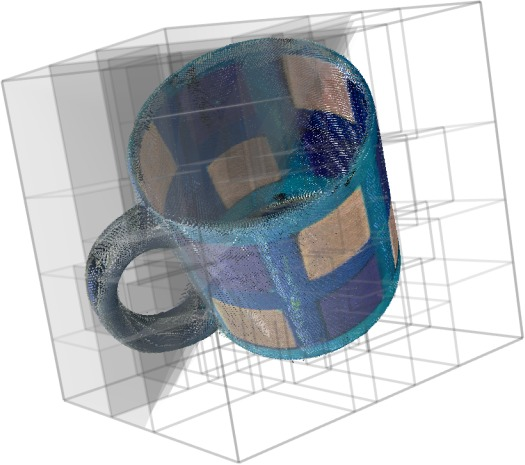
\includegraphics[width=0.65\textwidth]{localization-system/kdtree-3d}
		\caption[3-d tree]{3-d tree\protect\footnotemark}
		\label{fig:point-cloud-algorithms_3d-tree}
	\end{minipage}
	\footnotetext{\url{http://docs.pointclouds.org/trunk/group__kdtree.html}}
\end{figure}
\end{savenotes}
%}



\section{Reference map}

The reference point cloud can be loaded from a \gls{cad} file, point cloud file or dynamically arrive trough a \gls{ros} topic as either a 3 \gls{dof} occupancy grid or 6 \gls{dof} point cloud. This allows a localization supervisor to give only sections of a global map in order to use the least amount of memory and processing power (very large maps have deeper search structures, such as kd-trees, and should be avoided in order to improve the system efficiency).



\section{Point cloud assembly}

The laser assembler converts laser measurements in polar coordinates into Cartesian coordinates and projects the points using spherical interpolation in order to account for laser scan deformation that occurs when the robot is moving and rotating. It can merge scans from several lasers (sequentially or with a circular buffer) and it will publish the final point cloud after assembling a given number of scans or periodically after a specified duration. These assembly configurations can be changed at runtime through the use of the ROS dynamic reconfigure Application Programming Interface (API), which allows a localization supervisor to control the rate at which the localization system operates.



\section{Filtering and down sampling}

The time it takes to perform cloud registration is proportional to the amount of points in the ambient point cloud and in the reference map. As such, adjusting the level of detail of the point clouds by using voxel grids gives some control over the desired localization accuracy and the computational resources that will be required. This stage is also useful to mitigate the measurement errors of the depth sensors since the centroid of a voxel that contains points from several laser scans will be closer to the real surface (if the voxels have dimensions slightly larger than the expected laser measurement errors).

Point cloud data that comes from laser sensors can have a considerable amount of noise and an unnecessary level of detail. To cope with these problems, several preprocessing algorithms can be applied, ranging from simple point cloud downsampling to the more advanced outlier removal and surface reconstruction methods.


\subsection{Point cloud downsampling}

Downsampling methods aim to reduce the number of points while maintaining the surface structure of a given point cloud. They can be used to adjust the level of detail according to the point cloud registration precision required.


\subsubsection{Voxel grid sampling}

A voxel grid is a uniform space partition technique that can be used to cluster points according to their Euclidean coordinates. As can be seen in \cref{fig:point-cloud-algorithms_voxel-grid-downsampling}, it is a very effective method to control the level of detail of a point cloud because it gives the ability to specify the maximum number of points that a region in space should have.

The point cloud downsampling is achieved by replacing each cluster with a single point. The selection of this point can be very fast if the voxel center is used, but computing the centroid of the cluster yields better results because it represents the underlying surface with more accuracy and it attenuates errors in the sensors measurements.


%\afterpage{
\begin{figure}[H]
	\centering
	\begin{minipage}[h]{0.495\textwidth}
		\centering
			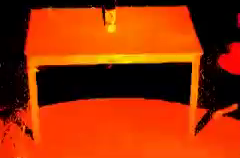
\includegraphics[width=0.78\textwidth]{localization-system/voxel-grid-downsampling-1}
	\end{minipage}\hfill
	\begin{minipage}[h]{.495\textwidth}
		\centering
	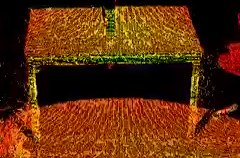
\includegraphics[width=0.78\textwidth]{localization-system/voxel-grid-downsampling-2}
	\end{minipage}
	\caption[Table point cloud before (left) and after (right) voxel grid downsampling]{Table point cloud before (left) and after (right) voxel grid downsampling\protect\footnotemark}
	\label{fig:point-cloud-algorithms_voxel-grid-downsampling}
\end{figure}
\footnotetext{\url{http://pointclouds.org/documentation/tutorials/voxel_grid.php}}
%}



\subsubsection{Random sampling}

Random sampling \cite{Vitter1984} is a fast downsampling method that randomly selects points from the input cloud until the specified number of samples is reached. This has the advantage of using real measures instead of downsampled approximations, but also means it is more sensible to sensor measurements noise. However, for outdoor environments or very complex scenes, using the real measurements can be preferable than using cluster centroids because the voxels may not have the necessary resolution or may have a prohibitive computational cost.


\subsection{Outlier removal}

Laser range finders can perform measurements with millimeter accuracy, but they have some limitations that can lead to the creation of outliers \cite{Sotoodeh2006}.

One of those limitations can produce shadow points around objects boundaries. This is due to the fact that a portion of the laser beam may hit the object boundary and other part may hit other areas in the object background. And given that most laser range finders use a weighted sum of several beams, this can yield measurements that are not associated with any real object (outliers). \Cref{fig:point-cloud-algorithms_voxel-grid-downsampling} shows a considerable amount of these shadow points close to the front table legs. Another issue is related to the angle in which the laser beam hits the objects. If the incidence angle is very low, then it may be difficult to detect if the beam had ambient reflections. This can significant increase the measurements noise or even lead to the creation of outliers. Other less common problem is associated with the material properties of the surfaces. For example, objects with very high or very low reflectance, such as metals or glass, can increase the measurements noise. Moreover depending on the combination of surface geometry, material and incidence angle, some objects may even be undetectable by laser range finders.

Given the negative effect that outliers have in object segmentation and registration algorithms, they should be removed in a preprocessing stage. There are several approaches to perform outlier detection and removal \cite{YangZhang2010}, ranging from simple distance thresholds to more robust statistical analysis. The next sections present some of then that can be useful in a localization system.


\subsubsection{Distance filter}

Given that laser range finders have a maximum distance for their measurements, it is wise to remove points that are close or beyond this limit. Moreover, it may be useful to remove points that are too close to the sensor, because they may belong to the robot itself and not the environment.

This can be achieved by applying a minimum and maximum threshold to the distances returned by the laser sensor (before converting then to Euclidean points).


\subsubsection{Passthrough filter}

A passthrough filter can select or remove points according to their properties.

For outlier removal, it can be used to select points that are within a given bounding box (useful when we already know what area of the environment we want to analyze) or remove points that don't have the appropriate intensity or color.


\subsubsection{Radius outlier removal filter}

The radius outlier removal filter deletes points that don't have a minimum number of neighbors within a specified radius distance. It can be useful when the point density is known and is very effective in removing isolated points.


\subsubsection{Statistical outlier removal filter}

The statistical outlier removal filter \cite{Rusu2010a} performs a global analysis of the distances between points and discards the ones that don't follow the global distance distribution.

It is a robust filter that adapts itself to the point cloud density and is very effective in removing shadow points. To do so, it computes the mean distance that each point has to a given number of neighbors and builds a global distance distribution (example in \cref{fig:point-cloud-algorithms_statistical-outlier-removal}). Then, assuming that the distribution is Gaussian, it discards the points that have a distance higher than a given threshold (that is a percentage of the standard deviation of the distance distribution).

%\afterpage{
\begin{figure}[H]
	\centering
	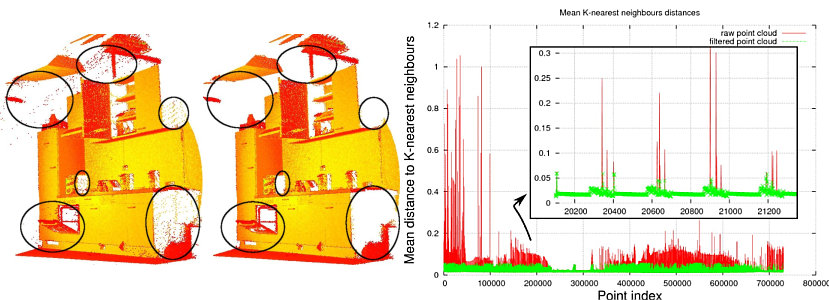
\includegraphics[width=\textwidth]{localization-system/statistical-outlier-removal}
	\caption[Statistical outlier removal filter]{Statistical outlier removal filter\protect\footnotemark}
	\label{fig:point-cloud-algorithms_statistical-outlier-removal}
\end{figure}
\footnotetext{\url{http://pointclouds.org/documentation/tutorials/statistical_outlier.php}}
%}


\subsection{Surface and object reconstruction and resampling}

Depending on the level of sensor noise and amount of outliers present in a given point cloud, it may be necessary to employ surface reconstruction techniques to fill gaps in sensor data or correct measurements errors. The next sections introduce some of the most common techniques to achieve these goals.


\subsubsection{Moving Least Squares}\label{sec:point-cloud-algorithms_mls}

Moving least squares \cite{Alexa2003} is a surface reconstruction algorithm that uses higher order bivariate polynomials to fit surfaces to a given set of points. It can be used to fill possible gaps in sensor data, smooth the point cloud (shown in \cref{fig:point-cloud-algorithms_mls-smoothing}), refine surface normals (shown in \cref{fig:point-cloud-algorithms_mls-nomal-refinement}) and perform downsampling or upsampling.

Surface reconstruction can also be useful when the point cloud is built from several laser scans with different origins and registered with some alignment errors. In \cref{fig:point-cloud-algorithms_mls-nomal-refinement} can be seen that the normal estimation is not very accurate in the regions of overlap between different scans. This can be solved by estimating the normals using the surfaces computed by the moving least squares algorithm instead of using the point's neighbors.


%\afterpage{
\begin{figure}[H]
	\centering
	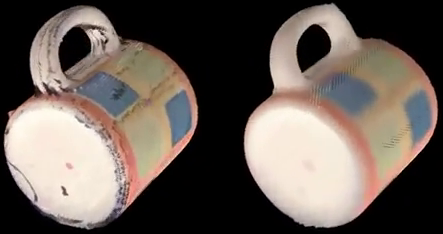
\includegraphics[width=0.57\textwidth]{localization-system/mls-smoothing}
	\caption[Surface smoothing using moving least squares algorithm]{Surface smoothing using moving least squares algorithm\protect\footnotemark}
	\label{fig:point-cloud-algorithms_mls-smoothing}
\end{figure}
\footnotetext{\url{http://pointclouds.org/documentation/tutorials/resampling.php}}
%}

%\afterpage{
\begin{figure}[H]
	\centering
	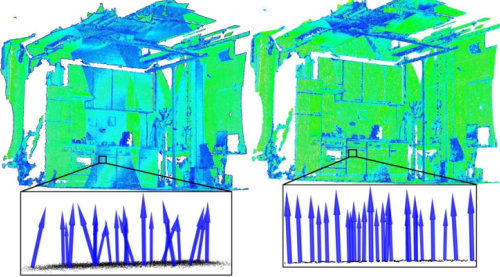
\includegraphics[width=0.57\textwidth]{localization-system/mls-nomal-refinement}
	\caption[Surface normals refinement using moving least squares algorithm]{Surface normals refinement using moving least squares algorithm \cite{Rusu2010a}}
	\label{fig:point-cloud-algorithms_mls-nomal-refinement}
\end{figure}
%}



\section{Normal estimation}

Most of feature detection, description and matching algorithms along with some registration methods rely on the point’s surface normal and curvature. As such, it was developed a robust 3 DoF normal estimation algorithm that uses Random Sample Consensus (RANSAC) [14] to fit lines to the sensor data and then orient the normals to the sensors origin. For 6 DoF data, the Principal Component Analysis (PCA) [15] or the Moving Least Squares (MLS) [16] approaches available in PCL can be used.


\subsection{3D surface normal estimation}

Surface normals provide information about the orientation of their underlying geometry and are widely used as the basis for other point descriptors. They can be computed using plane fitting methods or using more advanced techniques such as the one presented in \cref{sec:point-cloud-algorithms_mls}.

These algorithms analyze the neighborhood of a given point in order to compute the surface normal, and as such, the correct specification of what points should be included in the estimation is crucial to achieve accurate results. This depends on the environment geometry and the level of detail that is required, and is usually done by specifying a radius distance (example in \cref{fig:point-cloud-algorithms_surface-normals}) or by limiting the number of neighbor points to use.

\begin{figure}[H]
	\centering
	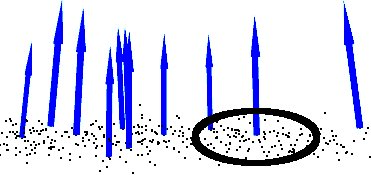
\includegraphics[width=0.5\textwidth]{localization-system/surface-normals}
	\caption[Point neighborhood for normal estimation]{Point neighborhood for normal estimation \cite{Rusu2010a}}
	\label{fig:point-cloud-algorithms_surface-normals}
\end{figure}


\subsection{2D normal line normal estimation}

FF.



\section{Keypoint detection}

Keypoint detection aims to find interesting points in a given point cloud in order to compute the cloud registration faster or to perform feature description and matching. There are several approaches to find keypoints that have different definitions of what kind of points are worth analyzing. But they all should be able to detect the same keypoints given similar data and they aim to select the points that best describe the underlying point cloud geometry. Currently the localization system can use the Scale Invariant Feature Transform (SIFT) [17] algorithm on the points curvature or the Intrinsic Shape Signatures (ISS3D) [18] keypoint detector.


Aligning two point clouds with overlapping views of the environment requires the establishment of point correspondences. If both point clouds have similar sensor origins, these can be determined with nearest neighbor's searches and filtered with correspondence rejectors (using other point properties such as reflectance and color). But if they were acquired in two very different positions, then more advanced techniques must be employed.

One of those techniques uses histograms to describe the geometric properties of the environment around a given point. This allows points to be matched even if they have completely different Euclidean coordinates. Also, by using histograms and sampling techniques, these descriptors are much more robust against sensor noise and varying level of point density. However, these advantages come with a heavy computational cost, and as such, point descriptors should only be computed on the most descriptive areas of the environment.

Identifying these environment points is known as feature / keypoint detection, and usually involves finding interesting points, such as corners and edges. Besides uniqueness, these points must also be repeatable. This means that the detection algorithms should be able to find the same points even if they are present in different point clouds with sensor noise and varying point density. This is of the utmost importance, because if the same keypoints are not identified on both clouds, then matching the point descriptors will likely fail.

The next sections introduce some of the most used algorithms for normal estimation, keypoint detection and point description.


\subsection{Intrinsic Shape Signatures}

FF.


\subsection{SIFT keypoints}

FF.



\section{Keypoint description}

Describing a keypoint usually involves analyzing its neighboring points and computing a given metric or histogram that quantifies the neighbor’s relative distribution, their normals angular relation, associated geometry or other metrics that are deemed useful. Several approaches were suggested over the years according to different recognition needs and they are the basis of feature matching algorithms used in the initial pose estimation.

The localization system can use most of the keypoint descriptors available in PCL, namely the Point Feature Histogram (PFH), the Fast Point Feature Histogram (FPFH), the Signature of Histograms of Orientations (SHOT), the Shape Context 3D (SC3D), the Unique Shape Context (USC) and the Ensemble of Shape Functions (ESF).


\subsection{Point Feature Histograms}

FF.


\subsection{Fast Point Feature Histograms}

FF.


\subsection{Shape Context Estimation}

FF.


\subsection{Unique Shape context}

FF.


\subsection{SHOT estimation}

FF.


\subsection{Spin image estimation}

FF.


\subsection{Ensemble Shape Functions}

FF.


\subsection{Rotational Projection Statistics}

FF.


\section{Cloud registration}

Point cloud registration is the process of finding the transformation matrix (usually translation and rotation only) that when applied to a given ambient cloud will minimize an error metric (such as the mean square error of the ambient point cloud in relation to a given reference point cloud). Several approaches were suggested over the years and they can be categorized as point or feature cloud registration.



\section{Initial alignment with keypoint descriptors matching}

Feature registration is the process of matching keypoint descriptors in order to find an initial alignment between two point clouds. The proposed localization system uses a feature registration method similar to the Sample Consensus Initial Alignment algorithm presented in [20]. It uses a sample consensus approach to select the best registration transformation after a given number of iterations. In each iteration a subsample of randomly selected descriptors from the ambient cloud is retrieved. Then for each of these descriptors, k best matching descriptors in the reference point cloud are searched and one of them is chosen randomly (this improves robustness against noise in the sensor data and changes in the environment that are not yet integrated into the map). Later after having filtered these correspondences between ambient and reference descriptors, the registration matrix is computed. If this registration matrix results in a point cloud overlap that has a minimum of inliers percentage (a point in the ambient cloud is an inlier if it has a point in the reference cloud closer than a given distance), then it is considered an acceptable initial pose and is saved (to allow a localization supervisor to analyze the distribution of the acceptable initial poses). In the end of all iterations, the best initial pose (if found) is refined with a point cloud registration algorithm.



\section{Final alignment with point cloud error minimization}

Point cloud registration algorithms such as the Iterative Closest Point [19] (with its several known variations like ICP point-to-point, ICP point-to-point non-linear, ICP point-to-plane and generalized ICP) and the Normal Distributions Transform [6] are among the most popular algorithms to register point clouds. They can achieve very accurate cloud registration but they require an approximate initial pose for the registration to successfully converge to a correct solution (otherwise they may achieve only partial cloud overlap or even fail to converge to a valid solution). To solve this problem, a complete autonomous registration pipeline must also include the computation of this initial alignment through the usage of feature registration.


\subsection{Iterative Closest Point}

FF.


\subsection{Normal Distributions Transform}

FF.



\section{Outlier detection}

FF.




\section{Localization validation}

After a point cloud is registered, several metrics are calculated in order to evaluate if a valid pose can be retrieved using the registration matrix.

The first computed metrics are the percentage of inliers and the root mean square error of these inliers. If a minimum number of points was registered and the inlier percentage and root mean square error are acceptable, then the registration is considered successful. However, these registered points can be agglomerated in a small area and may not be representative of the robot location. As such, a second metric is computed that takes into account the angular distribution of these inliers. This metric gives a measurement of how reliable is this registration and is based on the fact that there is high confidence in a given estimation when there are correctly registered points all around the robot.

The last metrics are the corrections that the registration matrix introduced. Given that the localization system will be in tracking mode most of the time, it is possible to define how far a new pose can be in relation to the previous accepted location and discard new poses that exceed a given threshold. This is useful to discard pose corrections that are very unlikely to happen, such as the robot moving half a meter between poses when it is expected to move only at 30 cm/s. These situations can happen when there is a sudden decrease in the field of view (that can occur due to sensor occlusion or malfunction) or when  large unknown objects very similar to sections of the map appearinto the field of view of the robot.

If all these metrics are within acceptable thresholds, then the robot pose can be computed by applying the matrix correction to the initial pose associated with the ambient sensor data. If any of these metrics are not acceptable, then the system can be configured to simply discard this pose estimation and try to estimate the pose in the next sensor data update or it can apply a tracking recovery attempt with a different registration algorithm (or the same algorithm with different parameters). If several consecutive pose estimations are discarded, the system can have a second level of recovery that can be configured to use the initial pose estimation algorithms in order to finally estimate the robot pose and reset the tracking state.



\section{Dynamic map update}

After performing a successful pose estimation, the localization system can be paired with OctoMap [21] in order to update the localization map by either integrating only the unknown objects or the full registered point cloud. Integrating only the unknown objects is the recommended approach when there is a known map and the environment is expected to change gradually. This is also more efficient as only the points that need to be integrated are processed and ray traced in OctoMap. On the other hand, integrating the full registered cloud can be desirable if the map of the environment is very incomplete, very outdated or expected to change considerably during the operation of the robot.
